\documentclass[a4paper, 12pt]{article}

% basic package list
\usepackage[T1]{fontenc}
\usepackage{fontspec}
\defaultfontfeatures{Mapping=tex-text}
\usepackage[margin=25mm]{geometry}
\usepackage{amsmath}
\usepackage{amsfonts}
\usepackage{amssymb}
\usepackage{graphicx}
%\setmainfont{???}

% other packages
\usepackage{xunicode}
\usepackage{xltxtra}
\usepackage{hyperref}         % hyperlinks
\usepackage{booktabs}         % professional-quality tables
\usepackage{indentfirst}      % to indent section first paragraph
\usepackage{url}              % simple URL typesetting
\usepackage{natbib}
\usepackage[modulo]{lineno}
\usepackage{sectsty}          % to change section font size
\usepackage[flushleft]{threeparttable} % table with note
\usepackage{caption}
\usepackage{lineno}

% set additional parameters
\setcitestyle{authoryear,open={(},close={)}}
\graphicspath {{Figures/}}

\sectionfont{\fontsize{14}{19}\selectfont}
\subsectionfont{\fontsize{12}{17}\selectfont}
\linenumbers

% Keywords command
\providecommand{\keywords}[1]
{
  \small	
  \textbf{\textit{Keywords---}} #1
}

%\newcommand{\beginsupplement}{%
%        \setcounter{table}{0}
%        \renewcommand{\thetable}{S\arabic{table}}%
%       \setcounter{figure}{0}
%        \renewcommand{\thefigure}{S\arabic{figure}}%
%     }

\title{Joint inference of adaptive and demographic history from temporal population genomic data}
\author{Vitor A. C. Pavinato$^1$, Stéphane de Mita$^2$, Jean-Michel Marin$^3$, \\
			Miguel Navascués$^1$$^*$}
\font\myfont=cmr12 at 10pt
\date{{\myfont %
    $^1$UMR Centre de Biologie pour la Gestion des Populations, INRAE, France\\%
    $^2$UMR Interactions Arbres-Microorganismes, INRAE, France \\%
    $^3$UMR Institut Montpelliérain Alexander Grothendieck, Université de Montpellier, France\\%  
    $^*$corresponding author: miguel.navascues@inra.fr\\[2ex]%
    }
    \today    
}
\begin{document}
\maketitle

\begin{abstract}
In evolutionary biology studies, there is a growing interest in using temporal genetic data (samples taken from many time-points) to understand how evolutionary forces interact in shaping the genetic diversity. Most of the methods available for analyzing temporal genomics data cannot completely address the interaction between demographic history and selection, while estimating parameters such as the effective population size $N_{\mathrm{e}}$ and the selection coefficient $s$ of adaptive variation. When selection is taken into account, these methods modeled it as a classic hard sweep, when a rare beneficial mutation with strong selection coefficient arise and sweep to fixation. But none of them can characterize the genome-wide signature of selection when selection is frequent and neither take into account the recurrent hitchhiking (RHH) selective sweep on the inference of demography. Taking advantage of the new development in Approximate Bayesian Computation via random forests (ABC-RF), we were able to estimate genome-wide demographic and selection parameters. Our ABC-RF framework was able to produce an unbiased estimate of $N_{\mathrm{e}}$ in a range of selection intensities and frequencies, as well as provide estimates of selection dynamics, such as the amount selection and the rate of beneficial mutations. These results demonstrate the potential of ABC-RF to jointly infer demography and selection in temporal population genomics.
\end{abstract} \hspace{10pt}

% keywords can be removed
\keywords{Temporal data, Population genomics, Substitution load, Machine learning}

\newpage
\section*{Introduction}
The goal of population genomics studies is to understand how demography and adaptive history shape the genetic diversity of a species. The classical approach is to assume that the sign of demographic events (migration, population subdivision, population expansion or contraction, for example) can be found spread genome-wide and that the footprint of selection (mainly directional selection) can be found in localized regions, usually close to mutations under selection. Several methods for demographic inference have been developed to capture the genome-wide signal. These methods use different inferential approaches such as maximum likelihoods, Bayesian or Approximated Bayesian Computation (ABC) and one or more summary statistics (site-frequency spectrum, as in $\partial$a$\partial$i, and many as in ABC-based methods, or the full data (see \cite{Beichman:2018bx} for a review)). In contrast, methods developed to identify the footprint of selection search for locus-specific signals left by the beneficial mutation on nearby neutral mutations \citep{Tajima:1989un, Fay:2000dl, Kim:2004ih}. Under the classical hard sweep model, selection happens on a rare mutation that has a positive selection coefficient. Selection allows this mutation increases in frequency, and over time, it sweeps through the population until fixation, carrying the nearby neutral mutations \citep{Smith:1974cy,Kaplan:1989tm, Barton:2000fg}. The hitchhiking of the neutral mutations, during the sweeps, leaves a signal of low genetic diversity and great differentiation that is then used to localize the beneficial mutation \citep{Nielsen:2005kx, Pool:2010eh, Scheinfeldt:2013iz, Vitti:2013jp, Casillas:2017jv}.

It is not easy to tease apart the signals left by demography or selection, since they can produce similar patterns on the genetic diversity. A step-by-step approach is frequently used in order to achieve a practicable estimate of demography or selection. First, a genome scan is performed to identify and remove outliers from the dataset before the demography analysis; second, demography inferred with “neutral" markers is used as a baseline model in the search for a selection signal. However, recent findings show that this approach is problematic given the pervasive role of selection (either positive and negative)\citep{Sella:2009hs,Hernandez:2011dn,Charlesworth:2012ix,Harris:2018bm,Lange:2018fl}. In addition, not only mutations with strong selection coefficients are able to sweep, but also weakly and mild mutations. As the search for localized signals of selection assumes only  strongly selected mutations, the weak and mild ones are not identified in genome scans and, consequently, are treated as neutrally evolving mutations. These mutations can strongly bias the demographic inference \citep{Huber:2015cl, Pavlidis:2010bb, Ewing:2016gv}, for example, overestimating the degree of population decrease.On the other hand, since genome scan methods are not robust to misspecifications of demographic history, an unspecified bottleneck or population increase, can inflate the type I error rate of genome scans \citep{Jensen:2005ky, Jensen:2007jw, Schrider:2016gg}. These results highlight the need for inferential methods that can take into account the multiple evolutionary processes that jointly act on populations \citep{Lin:2011jv, Li:2012bh, Bank:2014hx}. Advances in demographic inference were made when background selection (selection that acts on deleterious mutations) was taken into account \citep{Johri:2019jv}. But, the effects of positive and background selection are not similar, especially when more realistic models of BS are considered \citep{Schrider:2019ih}.

Approximate Bayesian Computation (ABC) has been proposed as a promising method for the jointly inference of demography and selection \citep{Li:2012bh, Johri:2019jv}. Initially proposed as a step-wise approach to infer selection \citep{Bazin:2010dv}, a first step with a wide prior distribution was used to estimate the effective population size $N_{\mathrm{e}}$ and the limits of the other parameters of the simulation. These limits and the estimated $N_{\mathrm{e}}$ were used on a second step to simulate neutrally and non-neutrally evolving mutations. By comparing the simulated trajectory of non-neutral mutations with the observed data through summary statistics, \citet{Bazin:2010dv} were able to obtain posterior estimates of the selection coefficients. \citet{Foll:2014kv, Foll:2015ce} formalized a framework, but replaced the first ABC step to estimate $N_{\mathrm{e}}$ by calculating a summary statistics directly in the data. This is problematic since the $N_{\mathrm{e}}$ estimate is naturally biased. In addition, they simplified the selection dynamics by simulating independent loci in their second step. The simulation of independent genetic loci was chosen in order to simplify the coalescent simulation used in their approach. However, it limits the simulation of complex selection dynamics of background selection and recurrent hitchhiking sweeps. An alternative to this, is the use of forward-in-time simulations \citep{Haller:2017gm}. However an implementation of a traditional ABC framework with forward-in-time simulations is unrealistic, given that an ABC regression algorithm requires a large number of simulations to produce reliable estimates of target parameters. The introduction of random forests in ABC reduced the computational burden, allowing the study of complex dynamics with few simulations \citep{Pudlo:2016il, Raynal:2017wm}.

Here, we present the development of an Approximate Bayesian Computation - Random Forests (ABC-RF) framework to jointly characterize the footprints of demography and positive selection on time-series genomic data. Population genetics studies generally make use of samples collected in one particular time-point to infer the role of drift and selection. However, developments in the area of ancient DNA \citep{Racimo:2016ea} and experimental evolution \citep{Barghi:2019gw,Kofler:2014if} have popularized the use of temporal genomic data. Their popularity influenced the development of methods and frameworks that better handle time-spaced allele frequency data (for a review \citet{Malaspinas:2015do}) and model the complex dynamics of selection and demography\citep{Malaspinas:2015do, FerrerAdmetlla:2016jc,Schraiber:2016ks}. Despite these advancements, in some methods, the $N_{\mathrm{e}}$ is considered a ``nuisance parameter'' (a parameter estimated by the model but not the main focus [citation]), mutations are modeled as evolving independently, neglecting the effects of linked selection \citep{Bollback:2008br, Malaspinas:2012dv,Feder:2014fe,Schraiber:2016ks, FerrerAdmetlla:2016jc}, and the global signature of selection and demography are not inferred.

In our framework, we made use of forward-in-time simulations which allowed us to model the complex dynamics of linked selection of beneficial mutations \citep{Haller:2017gm}. In our simulations, we were also able to model selection more generally with weakly to strongly selected mutations in scenarios that approximate to the classical hard sweep, where few beneficial mutations are present, and to scenarios of recurrent hitchhiking (RHH) sweep, where selection is more frequent. In our approach, demography was characterized directly with the estimates of the $N_{\mathrm{e}}$, the population census size $N_{\mathrm{cs}}$, the scale population size $\theta$, and the ratio between $N_{\mathrm{e}}$ and $N_{\mathrm{cs}}$. In all parameters, the global effect of selection was taken into account, which allowed us to obtain unbiased estimators. Selection was characterized globally by the genome-wide effect that it has on the genome. We were able, for the first time, to estimate the proportion of mutations under selection segregating in the population, as well as the rate at which beneficial mutations arise. This information is complementary to the methods developed to identify locus under selection and can be used in combination to better understand the evolutionary dynamics.

\section*{Methods}
\subsection*{Overview of ABC-RF}
Approximate Bayesian Computation (ABC) is a likelihood-free framework that compares the similarities between the real and simulated data generated from a given model \citep{Beaumont:2002ue}. Similarities between real and simulated data are evaluated by calculating the distance metric between a summary statistic that is obtained for each data. Usually, a tolerance level is defined and used to discriminate simulated data. Datasets and their associated values that are used to produce the simulations are kept if they are within the tolerance level and discarded if they are not. Posterior distribution is constructed for each parameter using the values kept for selected simulations \citep{Beaumont:2010gg}. The ABC method is consistent in estimating the true parameter behind the data if the sample size and number of simulations increase to infinity and the tolerance level decreases to zero  \citep{Frazier:2018kq}. In addition, even with a large number of simulations, two sources of subjectivity are always present using traditional ABCs algorithms: 1) choosing a tolerance level to accept/reject prior values, and 2) choosing a summary statistic to make acceptance and rejection decisions. 

A major advancement in ABC's inference came with the introduction of Random Forests (RF)\citep{Pudlo:2016il,Raynal:2017wm}. RF is an algorithm that learns from a database (here referred to as ``reference table'') how to predict the value of a parameter $q$ of an independent dataset. The reference table is produced by combining the parameter values of the simulations and the values of summary statistics calculated on the simulated data. This reference table can be used to train an algorithm capable of estimating parameters or selecting which model can generate the patterns observed in the real data. The parameter estimation and model selection is done by comparing the summary statistics of the observed data with the simulated data using decision trees (for more information about ABC-RF \citet{Pudlo:2016il} and \citet{Raynal:2017wm}). The main advantage of using ABC-RF for the inference of demography and selection is that it requires less simulation for reliable classification \citep{Pudlo:2016il, Fraimout:2017jq} and posterior estimates \citep{Raynal:2017wm}. It is important to reduce the number of simulations because the complex dynamics of demography and selection can only be simulated with forward-in-time simulations, which are computationally expensive. The second advantage of the ABC-RF is that it reduces subjectivity in choosing summary statistics and eliminates the definition of tolerance thresholds.

\subsection*{ABC-RF framework for joint inference of adaptive and demographic history}

For the joint inference of adaptive and demographic history within the ABC-RF framework, our model consisted of a single population of diploid individuals of constant size, sampled at two time-points. In our model, beneficial mutations can originate in the population in any generation. The model was divided into two phases 1) a ``burn-in phase'' consisting of a number of generations performed by simulations to minimize the effect of initial conditions, and 2) a ``sampling phase'' containing the time-interval (in generations) of the first and second samples of individuals. The parameters of the model are the population census size of the burn-in phase (phase 1 from now on) $N_{\mathrm{cs}1}$, the population census size for the sampling phase (phase 2 from now on) $N_{\mathrm{cs}2}$, the mutation rate per generation $\mu$, the per base recombination rate per generation $r$, the proportion of selected mutations $P_{\mathrm{S}} = P_{\mathrm{R}}P_{\mathrm{B}}$ (where $P_{\mathrm{R}}$ is the proportion of non-neutral regions and $P_{\mathrm{B}}$ is the probability that a beneficial mutation will arise in a non-neutral region), and the mean of the gamma distribution $\kappa\theta$ that defines the values of the selection coefficients $s$ of beneficial mutations (it can also be called the distribution of fitness effects - DFE) (supplementary Methods S2 has more details about the model).

The objectives of the ABC analysis would be to infer each of the above parameters from the model. However, except for population census size of the second period $N_{\mathrm{cs}2}$, the parameters were treated as ``nuisance parameters'' that are used to generate allele frequency trajectories of linked and unlinked neutral and beneficial mutations. Our goal was to jointly characterize the adaptive and demographic history in between samples of the genetic data. In order to infer the overall effect of demography and selection, we infered the $N_{\mathrm{cs}2}$ (from now on called $N_{\mathrm{cs}}$ for simplification) and other seven latent variables: 1) the average genetic load $L$, that measures the overall diversity of beneficial mutations (substitution load); 2) the proportion of mutation under strong selection $P$ (where $s > 1/N_{\mathrm{e}}$); 3) the scale population size of beneficial mutation $\theta P_{\mathrm{S}}$ as it measures the rate at which beneficial mutations enter the system; 4) the population scaled selection coefficient $N_{\mathrm{e}}s$, a measurement of the distribution of fitness effects (DFE); 5) the effective population size $N_{\mathrm{e}}$, 6) the population scale population size $\theta$, and 7) the ratio between the effective population size $N_{\mathrm{e}}$ and the population census size $N_{\mathrm{cs}}$, $N_{\mathrm{e}}/N_{\mathrm{cs}}$, as it is a measurement of how the census size reflects the actual effective population size. In our model, as the only forces that were considered are selection and drift, we expect to have a dramatic reduction on $N_{\mathrm{e}}$ compared to $N_{\mathrm{cs}}$ when beneficial mutations are more frequent.

n every generation, the substitution load was calculated as a difference between the individual with the highest total fitness and the average overall fitness of the population at that generation $i$,  
\begin{gather*}
    L_{i} = \frac{W_{\mathrm{max}i} - \bar{W_{i}}}{W_{\mathrm{max}i}}
\end{gather*}

where $W_{\mathrm{max}}i$ represents the individual with the highest fitness in the population and $\bar{W_i}$ represents the average fitness of the population in the generation $i$. The average substitution load was obtained by averaging all values.

Since in our simulation we can track the selection coefficient $s$ of all mutations segregating in every generation $i$, we can obtain the fraction of mutations strongly selected in the period 2 as:  
\begin{gather*}
    P = \frac{\text{mutations with } s > 1/N_{\mathrm{e}}}{\text{all segregating mutations}}
\end{gather*}

The scale population size of beneficial mutation $\theta P_{\mathrm{S}}$ was calculate as: 
\begin{gather*}
    P = 4 N \mu P_{\mathrm{S}} G
\end{gather*}

where $P_{\mathrm{S}}$ is the composed parameters that control the amount of beneficial mutations in the simulation and $G$ is the genome size. The overall strength of selection was calculated as $N_{\mathrm{e}}s = N_{\mathrm{e}}\kappa\theta$, where $\kappa\theta$ is the mean for a gamma distribution. The effective population size $N_{\mathrm{e}}$ was calculated by the harmonic mean of each $N_{\mathrm{e}}i$ calculated in each generation $i$. Each $N_{\mathrm{e}}i$ was calculated as the average reproductive success of individuals in the population:
\begin{gather*}
    N_{\mathrm{e}}i = \frac{4N}{2+var(g_{i})} 
\end{gather*}
where $g_{i}$ represents the number of times each individual of the generation {$i$-1} contributed as a parent. From the harmonic mean of the effective population size, we calculated $\theta = 4N_{\mathrm{e}}\mu$.    

In addition, we used the simulations to test the ability of our ABC-RF framework to separate scenarios with selection from neutral scenarios. Our ABC-based classifier was trained to discriminate scenarios where beneficial mutations were either constant or limited, weak or strong. Based on the values of the latent variable $P$ (the proportion of mutation under strong selection) we defined two discrete classes of scenarios: 1) quasi-neutral scenarios where the proportion $P=0$; and 2) strong selection scenarios where $P > 0$.

Simulation with different values for the model parameters were used to make inferences about the parameters and latent variables that describe the overall pattern of demography and selection. For each simulation, values of the model parameters were sampled from each parameter' prior distribution and used to simulate a forward-in-time dynamic of selection. Simulations were performed with the software SLiM v3.1 \citep{Haller:2017gm, Haller:2018gn}. SLiM is an efficient forward-in-time simulator based on the extended Wright-Fisher model, and it can simulate complex dynamics, as non-neutral selection acting on linked sites \citep{Messer:2013ct}. We divided our simulations into two periods, the burn-in and the sampling phase, to efficiently simulate the desired dynamics of selection. In the burn-in phase, we tracked when all the mutations lineages present in the simulation coalesced (\textit{initializeTreeSeq(checkCoalescence=T)}). By using it, we reduced the computational time required to finish a simulation, because the number of generations equal to 10*$N_{eq}$ was no longer required, especially with the dynamics of strong and frequent selection. The second phase of the simulation outputs genotypic data of a sample of individuals, such as single nucleotide polymorphis (SNPs), in the vcf file in two time-points. This data is combined with bcftools v.1.9 (\url{https://samtools.github.io/bcftools/}) and converted to fit a custom egglib script that calculates the summary statistics (Supplementary Methods S1.3). For every simulation, a reference table is produced by combining the model parameters, latent variables and the summary statistics. The reference table was used to estimate the posterior distribution using the R package abcrf \citep{Pudlo:2016il,Raynal:2017wm}. We implemented this approach into R scripts that we made available on github (\url{https://github.com/vitorpavinato/Tracking-selection/}). 

\subsection*{Simulations}

\begin{table}[ht]
 \caption{Simulation parameters and their prior distribution.}
  \centering
  \label{table:table1}
  \begin{tabular}{lll}
   \cmidrule(r){1-3}
    Parameter                                                    & Prior distributions                  & Parameter range\\
    \midrule
    Population size for the period 1                             & $N_{\mathrm{cs}1} \sim loguniform$   & 1 to 2,000\\
    Population size for the period 2                             & $N_{\mathrm{cs}2}  \sim loguniform$  & 1 to 2,000\\
    Mutation rate                                                & $\mu \sim loguniform$                & 1e-10 to 1e-6\\
    Recombination rate                                           & $r \sim loguniform$                  & 5*1e-7 to 5*1e-10\\
    Proportion of selected mutations $P_{\mathrm{S}}$:           &                                      &                  \\
        1) Proportion of non-neutral regions, $P_{\mathrm{R}}$   & $P_{\mathrm{R}} \sim uniform$        & 0 to 1\\
        2) Probability of beneficial mutation, $P_{\mathrm{B}}$  & $P_{\mathrm{B}} \sim loguniform$     & 1e-5 to 1\\ 
    Mean of Gamma distribution $\kappa\theta$                    & $\kappa\theta \sim loguniform$       & (1e-3 to 1)\\
    \bottomrule
  \end{tabular}
  \label{tab:tab1}
\end{table}

The method described above was evaluated on simulated data. In the simulations, each individual had a genome of size 100 Mb that was divided in 2,000 fragments of 50,000 bps. A number of these fragments were defined as either neutral or non-neutral, based on the parameter $P_{\mathrm{R}}$. Non-neutral regions harbored beneficial mutations given the probability $P_{\mathrm{B}}$. Dominance coefficients were set 0.5 for all mutations throughout the simulation. In the period 2, 100 individual genotypes were sampled in the first generation TS1, and 100 more after 10 generations (TS2). About 50,000 simulations were generated and used to train the ABC-RF. Table 1 shows the prior distribution set for each model parameter with the associated prior range used to produce the simulations. Additional 1,877 simulations were produced with the same priors and range to use as pseudo-observed data (from now on called ``random-parameter-values PODs''). We also produced PODs with fixed parameters that helped us explore the parameter space where the method has more inferential power and/or limitations (this PODs are called from now on ``constant-values PODs''). We defined the parameter values for neutral and non-neutral scenarios. For the non-neutral scenarios we varied the strength and amount of selection. The strength of selection was determined by the mean of the gamma distribution of the selection coefficients (0.01, 0.10, and 0.25), and the amount was determined by the rate of beneficial mutations ($1e-4$ and 0.20). The combination of strength and frequency of beneficial mutations allowed us to evaluate the performance of our method in in a scenario where adaptation is mutation limited, and where it is unlimited. In a mutation limited scenario, a beneficial mutation takes more time to appear (``hard sweep'' scenario, where the time lag for a beneficial mutation to arise is proportional to $s$). On the other hand, in a mutation unlimited scenario, in every generation a beneficial mutation can appear ($P_{\mathrm{S}}\theta > 1$. For each scenario, 100 replicated simulations were produced. For the calculation of the summary statistics (for simulations used to train the Random Forests and for simulations to evaluate it), we calculated locus-specific summary statistics with three window sizes: 500, 5,000 and 10,000 bp, and site-frequency spectrum with three bin sizes: 10, 15 and 20 bins.

In summary, the random PODs were used to ABC-RF in a range of possible combinations of parameters and parameter space to approximate what could happen when the degree of selection ranges from weak to strong. The ``constant-values PODs'', in contrast, allowed us to assess how the ABC-RF estimated the posterior values in fixed evolutionary scenarios of weak versus strong selection, where selection is rare or frequent. Keeping the parameters fixed allowed us to add a random noise, since the number of mutations and their trajectory for fixation or loss may vary due to the stochastic nature of the simulation.

\begin{table}[ht]
 \caption{Simulation parameters for the ``constant-values PODs''}
 \label{table:table2}
  \centering
  \begin{tabular}{llll}
   \cmidrule(r){1-4}
    Parameter                 & Neutral  & Mutation           & Mutation           \\
                              &          & limited            & unlimited           \\
    \midrule
    $\mu$                     & $1e-8$   & $1e-8$             & $1e-8$             \\
    $r$                       & $5.0e-8$ & $5.0e-8$           & $5.0e-8$           \\
    $N_{\mathrm{cs}1}$        & 500      & 500                & 500                \\
    $N_{\mathrm{cs}2}$        & 500      & 500                & 500                \\
    DFE $mean=\kappa\theta$   & NA       & (0.01, 0.10, 0.25) & (0.01, 0.10, 0.25) \\
    $P_{R}$                   & NA       & 0.25               & 0.25               \\
    $P_{S}$                   & 0        & $1e-4$             & 0.20               \\
    \bottomrule
  \end{tabular}
  \label{tab:tab2}
\end{table}

\subsection*{Dataset}

In addition to the PODs, one data-set from the literature was re-analyzed with our ABC-RF method. The dataset consisted of whole-genomic sequencing data from museum and contemporary specimens of feral populations of \textit{Apis mellifera}  collected in California from 1910 to 2011 \citep{Cridland:2018fx}. Our goal was to evaluate the performance of our framework to infer demography and selection parameters in a real data-set, and not to re-analyze the entire data-set. We selected one location containing one isolated population with five and six individuals collected in each time-point. Two samples of five whole-genomes spanning 15 years (or 15 generations assuming one generation/year) were taken at the Placerita Canyon Nature Area, in Los Angeles county, California, United States. For the simulations, we set the genome size of each individual as 250 Mb (similar to the most recent estimates of \textit{A. mellifera} genome size \citep{Elsik:2014hf}. The genome was divided into 5,000 fragments of 50,000 bps. As with the PODs, a number of these fragments was defined as neutral or non-neutral based on the parameter $P_{\mathrm{R}}$. Dominance coefficients were set 0.5 for all mutations throughout the simulation. In the period 2 (sampling period), five individual genotypes were sampled in the first generation (TS1), and five more after 15 generations (TS2). We produced 15,000 simulations to train the ABC-RF. We used a $log_{10}(Normal)$ distribution for the $\mu$ with mean 3.4e-9 with standard deviation of 0.5. The per base recombination rate was set as $log_{10}(Uniform)$ ranging from 1e-8 to 1e-4. The census size $N_{CS_{1}}$ and $N_{CS_{1}}$ were set with a $log_{10}(Uniform)$, ranging from 1 to 10,000 individuals. Other model parameters were set similarly to the PODs.

\section*{Results and Discussion}

\subsection*{Joint estimation of demography and adaptive history}

We evaluated if our ABC-RF approach was able to estimate parameters informative about demography while taking into account directional selection in hard \citep{Smith:1974cy,Kaplan:1989tm,Barton:2000fg} or recurrent hitchhiking (RHH) sweeps \citep{Lange:2018fl,Wiehe:1993cm}. In hard sweeps scenarios, a rare but strong beneficial mutation arises and sweeps to fixation. In RHH however, beneficial mutations are more frequent, randomly appearing in the genome. For this reason, the fixation path of each beneficial mutation depended not only on its selection coefficient, but also on the interaction between other selected mutations. The strength of these interactions was determined by the $N_{\mathrm{e}}$ and by the recombination rate - Hill-Robertson interference (HRI) \citep{Hill:2007gx,Neher:2013ju}. We did not simulate each scenario separately, but we allowed the dynamic to emerge as a function of the mutation rate of beneficial mutations. We also defined a wide range for selection coefficients, which allowed us investigate the effect of strong \citep{Jensen:2008eo} and mild and weak selection \citep{Lange:2018fl}.  

Our ABC-RF approach was able to estimate $N_{\mathrm{e}}$ (figure 1b) regardless the amount and the strength of beneficial mutations (Figure 1a). Figure 1b shows the distribution of the true and predicted value for the $N_{\mathrm{e}}$. The predicted values represent the ones obtained with the process of growing the random forests trees. The distribution of predicted values of each parameter was later used to obtain a posterior estimate of an observed data, comparing the summary statistics of the training data with the observed data. As we can see in figure 1c, the estimate of $N_{\mathrm{e}}$ based on the average $F_{\mathrm{ST}}$ were greatly impacted by selection. The overall $F_{\mathrm{ST}}$ represents the accumulated allele frequency changes between time-spaced samples. Assuming selective neutrality, the difference is determined only by drift, with this effect depending on the effective size of the population. With selection, however, divergence is determined by the combined effect of selection and drift. In a RHH scenarios, the pace of divergence depends on the amount of beneficial mutations sweeping, as it can quickly reduce the $N_{\mathrm{e}}$ \citep{Lange:2018fl}, increasing the effectively neutral mutation rate \citep{Walsh:2018tv}.

\begin{figure}[ht]
  \centering
  \label{fig:fig1}
  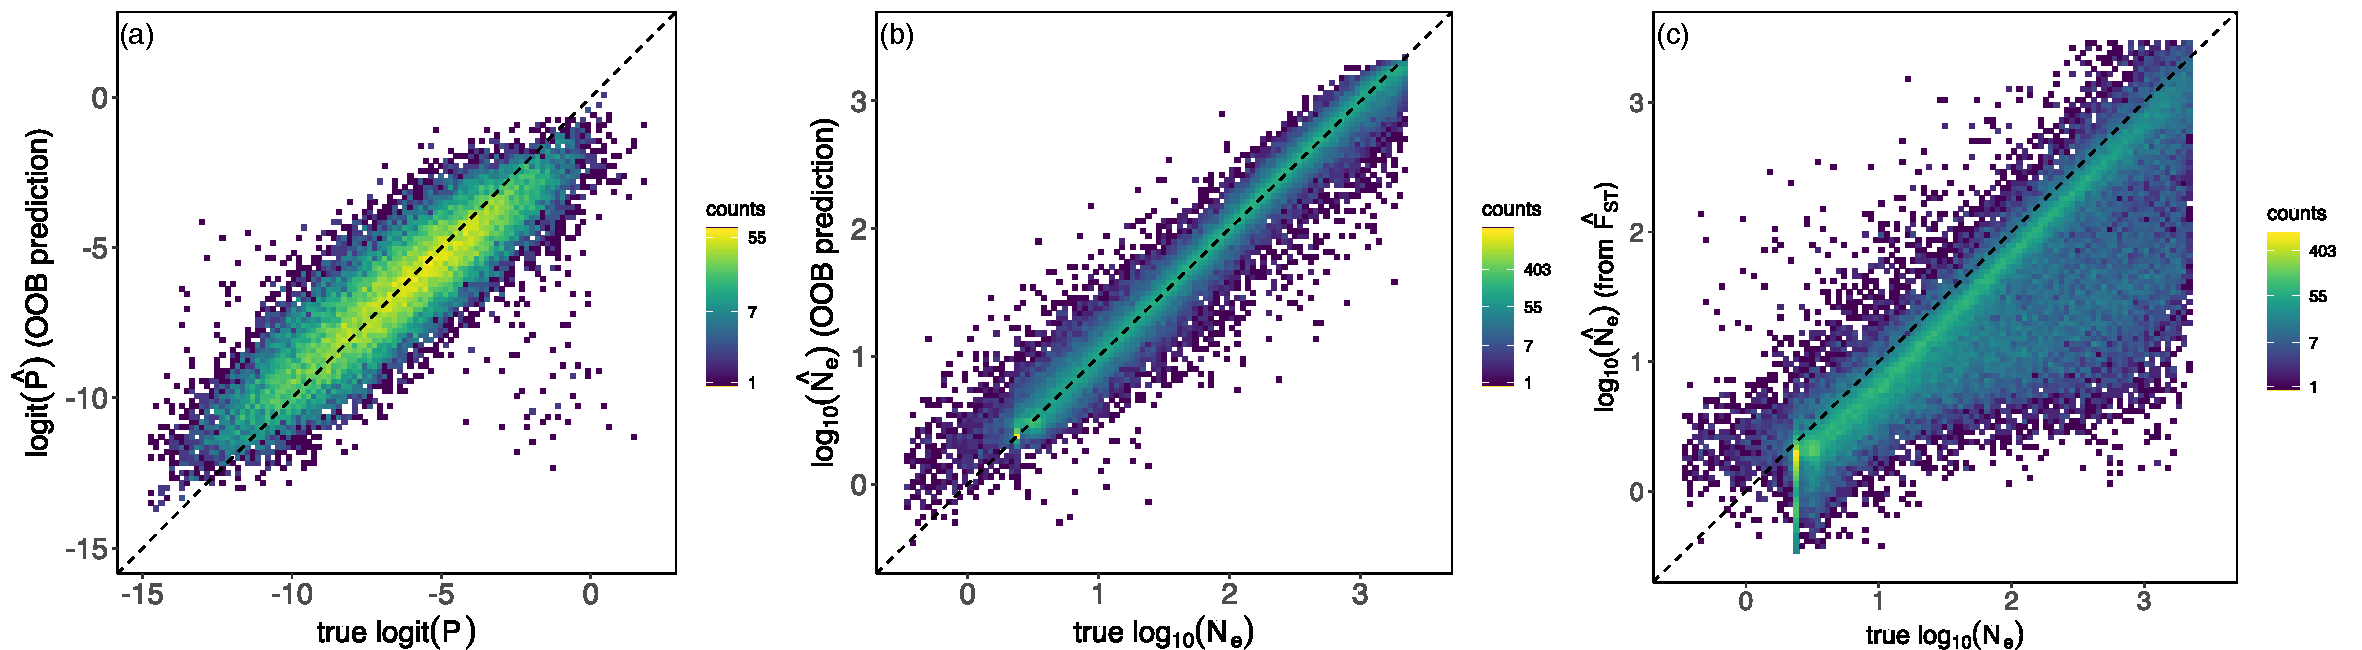
\includegraphics[width=1\textwidth]{Figures/joint_demosel_ggplot2_mod.pdf}
  \captionsetup{font=footnotesize}
  \caption{Joint inference of adaptive and demography history with ABC-RF. \textbf{(a)} the proportion of strongly selected beneficial mutations $P$, and \textbf{(b)} the effective population size $N_{\mathrm{e}}$ estimated with the ABC-RF; and \textbf{(c)} the $N_{\mathrm{e}}$ estimated with an estimator derived from the temporal $F_{\mathrm{ST}}$.}
\end{figure}

In figure 1a, we can also see that our method was able to jointly infer the proportion of strongly selected mutations segregating in the population. The fact that this latent variable quantifies only the proportion of mutation with $s > 1/N_{\mathrm{e}}$ do not remove the impact and interference of mild and weak selection that was present in the population. These mutations could leave an unpredictable signal on nearby neutral and beneficial mutations and, they could consequently impact the overall genetic diversity that as captured on the summary statistics.

In addition to the $P$, we also expanded our ABC-RF approach to estimate other parameters informative about adaptation history: a) the average substitution load $L$, that measures the impact of any beneficial mutation on the overall fitness of the population (this can also be interpreted as the overall diversity of selected mutations); b) the population scale parameter of the beneficial mutations $\theta P_{\mathrm{S}}$, that measures the rate at which  beneficial mutations emerge; and c) the population scaled selection coefficient $N_{\mathrm{e}}s$, that measures the distribution of fitness effects (DFE) of beneficial mutations. In order to grow the random forests for $P$ and $L$, simulations with no selection were removed from the training reference table. We used a logit transformation for the vector of each of these two parameters, and the $log_{\mathrm{10}}$ transformation for $\theta P_{\mathrm{S}}$ and $N_{\mathrm{e}}s$ (the distribution of each parameter used to grow the RFs can be found in supplement, Figure S2). 

Figure S3a to d shows the distribution of the true values versus the predicted values of the parameters and latent variables for the parameters informative about selection. The predicted values were similar to the expected (figure S3 a-d), but bias can be seen in the estimator for the substitution load and for the proportion of strongly selected mutations (Figures S4 a and b). The bias in $L$ reflects the limitation to estimate it in scenarios with limited selection, and the bias on $P$ corresponds to scenarios where selection was too intense, reducing $N_{\mathrm{e}}$ drastically and causing any beneficial selection, within the prior range, to be considered as neutral mutations.

For the demography, we also trained an ABC-RF to estimate the population census size $N_{\mathrm{cs}}$, the ratio between $N_{\mathrm{e}}$ and $N_{\mathrm{cs}}$, and population scale population size $\theta$. Overall, the parameters about demography were less biased (Figure S3 e, f and h), except the ratio between $N_{\mathrm{e}}$ and $N_{\mathrm{cs}}$ (Figure S3 g). The ratio $N_{\mathrm{e}}/N_{\mathrm{cs}}$ is an important measurement in conservation genetics because it tells us how well the population census size represents the effective size. For example, in a large and isolated population with constant population size and no selection, the $N_{\mathrm{e}}$ should be close to $N_{\mathrm{cs}}$. In the same scenario, but with few and strong beneficial mutations, the deviation of $N_{\mathrm{e}}$ from $N_{\mathrm{cs}}$ is small. In a scenario with RHH, however, we expect to have $N_{\mathrm{e}}$ far below the $N_{\mathrm{cs}}$, as a consequence of the drastic reduction on the $N_{\mathrm{e}}$ by selection. The bias we observed on this parameter reflects the fact that our model explored better the parameter space of strong and recurrent selection than the space of neutral/quasi-neutral scenarios and/or hard sweep scenarios.

An important feature of the ABC analysis with Random Forest is that we do not need to specify the summary statistics a priory, because the tree growth process classifies the most informative summary statistics for each parameter of interest. For example, for the $N_{\mathrm{e}}$ the mean $F_{\mathrm{ST}}$ across all locus-specific estimates was the most informative. On the other hand, for the substitution load, the skewness of the locus-specific $F_{\mathrm{ST}}$ was the most informative (Figure S4).

We evaluated the performance of the trained random forests by estimating the parameters of pseudo-observed data. We first evaluated them on the PODs that were generated with the same prior range as the simulation used to train the ABC-RF (from now on called random-parameter-values PODs). Note that the random-parameter-values PODs were not used to train the random forests, as these simulations were set aside before to be used only for testing the trained RF. As the random-parameter-values PODs covered the same parameters space as the training data, we had similar performances, except for $P$ and $L$ (Figure 2). For these latent variables, the inference on the test dataset was biased because neutral simulations were removed to generate the training set (Figure 2a and b).

\subsection*{The impact of adaptive dynamic on demography and selection inference}

We also evaluated the performance of the trained ABC-RF on PODs with fixed parameters that were used to emulate neutral, adaptation mutation limited and unlimited scenarios. With these  PODs, because we could control the amount and strength of selection, we could compare scenarios that approximate to a classical hard sweep (mutation limited) or to a recurrent hitchhiking (mutation unlimited). This was achieved by varying the rate at which each new beneficial mutation arises. When a new mutation has a low rate, the dynamics resembles a hard sweep model. On the other hand, when a beneficial mutation has a high rate and is allowed to appear to any position on the genome, even at the same position of an already existing beneficial mutation, the dynamics resembles a recurrent hitchhiking sweep. Within each evolutionary dynamics, we also evaluated the performance of our RF with three degrees of selection.

For adaptation in a mutation unlimited scenario, the ABC-RF recovered the true value for the selection parameters, regardless the strength of selection (Figure 3), except for $N_{\mathrm{e}s}$ where the ABC-RF overestimated with lower values and underestimated with higher values of mean $s$. For scenarios where adaptation is limited, the ABC-RF had difficulty to estimate the substitution load and the proportion of locus under selection, and underestimated the DFE for all strengths of selection. It is interesting that the parameter informative about the selection dynamic, $\theta P_{\mathrm{S}}$, is independent of the strength of selection. 

Overall, demographic were satisfactorily estimated with our ABC-RF approach. We can see more bias on the estimates of $N_{\mathrm{e}}$ and consequently on $N_{\mathrm{e}}/N_{\mathrm{cs}}$ in scenarios where adaptation is not limited by mutation, but only when the strength of selection increased. When selection increased, only the variance around the true value increased (Figure 4).  

\subsection*{Comparison with available methods to estimate $N_{\mathrm{e}}$}

It is not the first time that the impact of RHH on the $N_{\mathrm{e}}$ inference \citep{Lange:2018fl} was accessed in scenarios where selection ranged from weak to strong, however it is the first time that an unbiased estimate of $N_{\mathrm{e}}$ on RHH and classical sweep scenario is presented. By comparing our ABC-RF $N_{\mathrm{e}}$ estimates with the ones obtained with WF-ABC \citep{Foll:2014kv,Foll:2015ce} and with the temporal $F_{\mathrm{ST}}$ (Figure 5), we could see how the RHH dynamics impacts the $N_{\mathrm{e}}$ and how our model performed well regardless the strength and rate of selection. For the random-parameter-values PODs, both methods produced (on average) biased estimates, WF-ABC overestimating it and the temporal $F_{\mathrm{ST}}$ underestimating it. For the constant-values PODs, our ABC-RF was able to recover the true value of $N_{\mathrm{e}}$ regardless the amount and the strength of selection. But, the other two methods underestimated the $N_{\mathrm{e}}$ in mutation unlimited scenarios, more critically when the overall strength of selection was strong. For scenarios that approach the classic hard sweep model (mutation limited) however, both methods performed well, regardless the strength of selection. 

\begin{figure}[!htb]
  \centering
  \label{fig:fig2}
  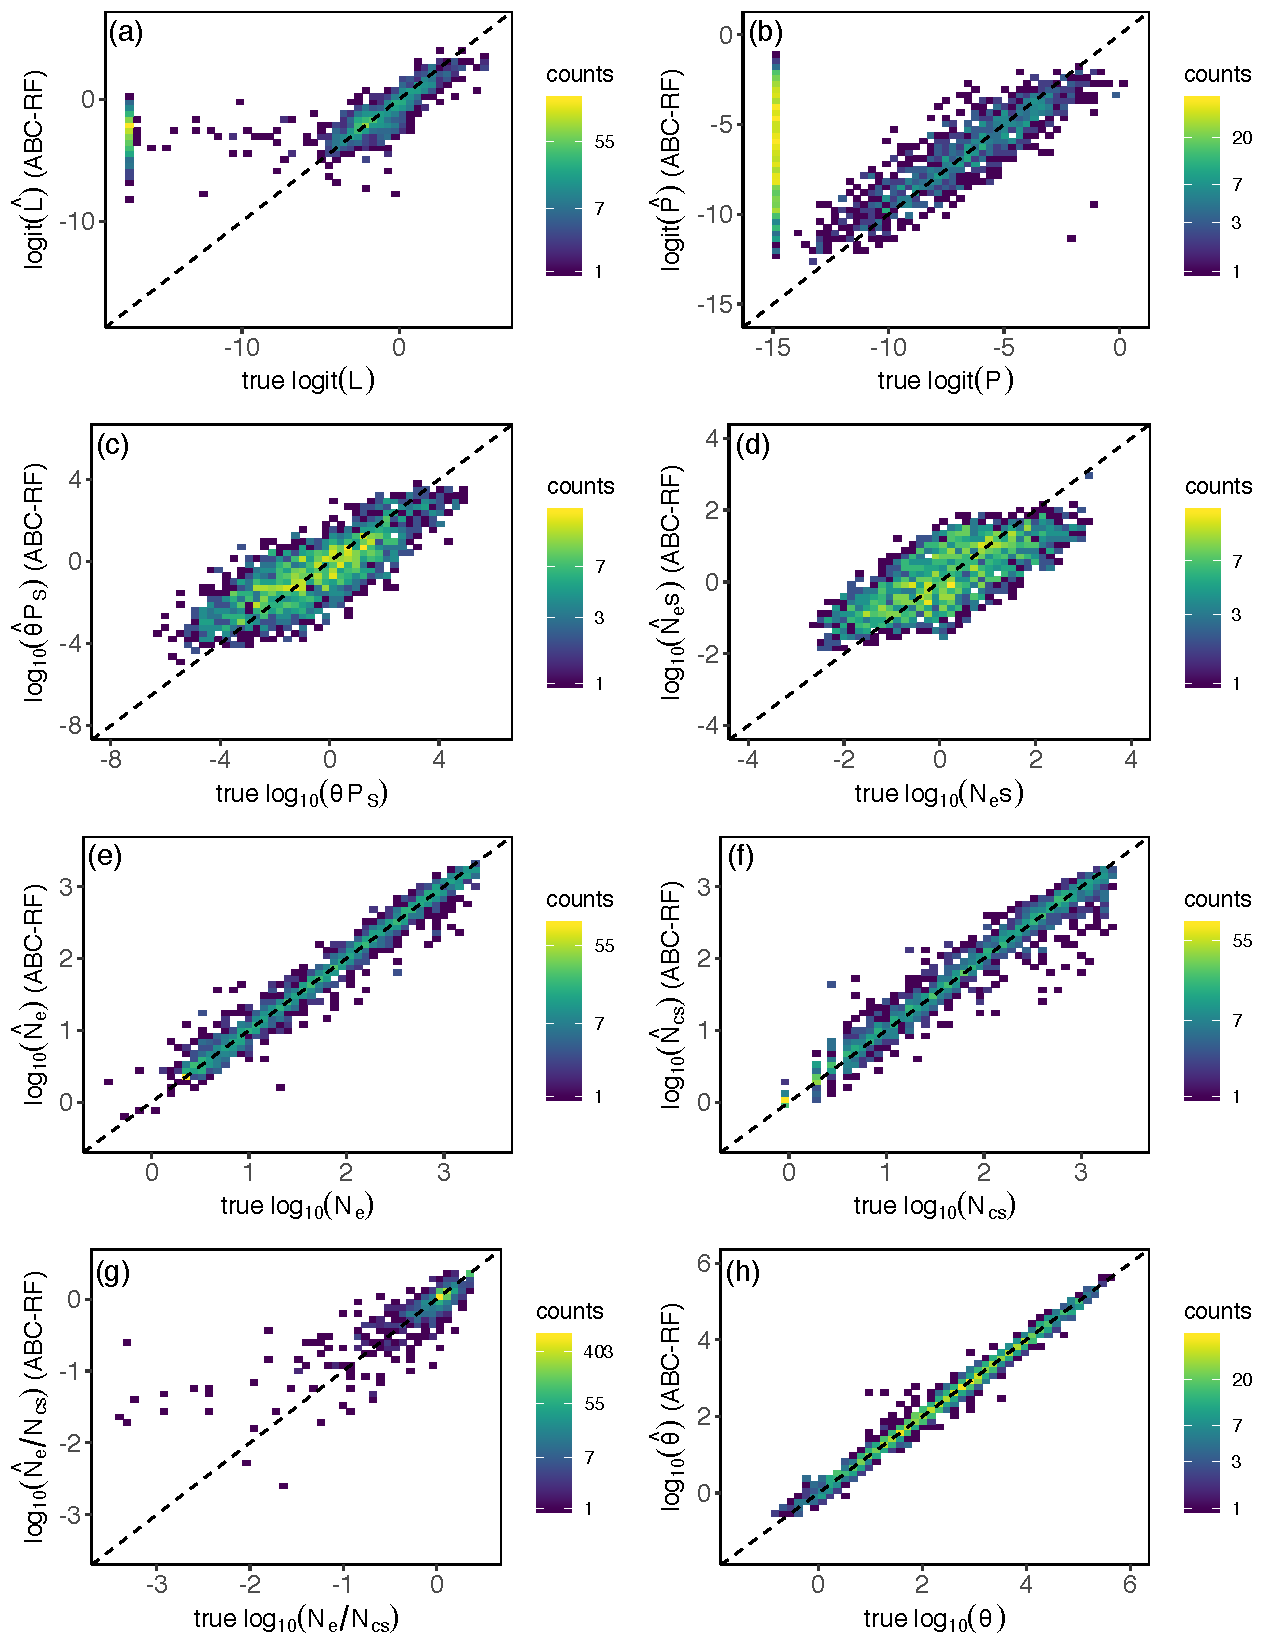
\includegraphics[width=1\textwidth]{Figures/pred_plots_ggplot2_mod.pdf}
  \captionsetup{font=footnotesize}
  \caption{Estimated parameters for the random-parameter-values PODs. \textbf{(a)} substitution load $L$; \textbf{(b)} proportion of strongly selected beneficial mutations $P$; \textbf{(c)} scale population size of beneficial mutation $\theta P_{\mathrm{S}}$; \textbf{(d)} overall strength of selection was calculated as $N_{\mathrm{e}}s$; \textbf{(e)} effective population size $N_{\mathrm{e}}$; \textbf{(f)} population census size $N_{\mathrm{cs}}$; \textbf{(g)} ratio between the effective size and the population census size; and \textbf{(h)} scale population size $\theta$.}
\end{figure}

\begin{figure}[!htb]
  \centering
  \label{fig:fig3}
  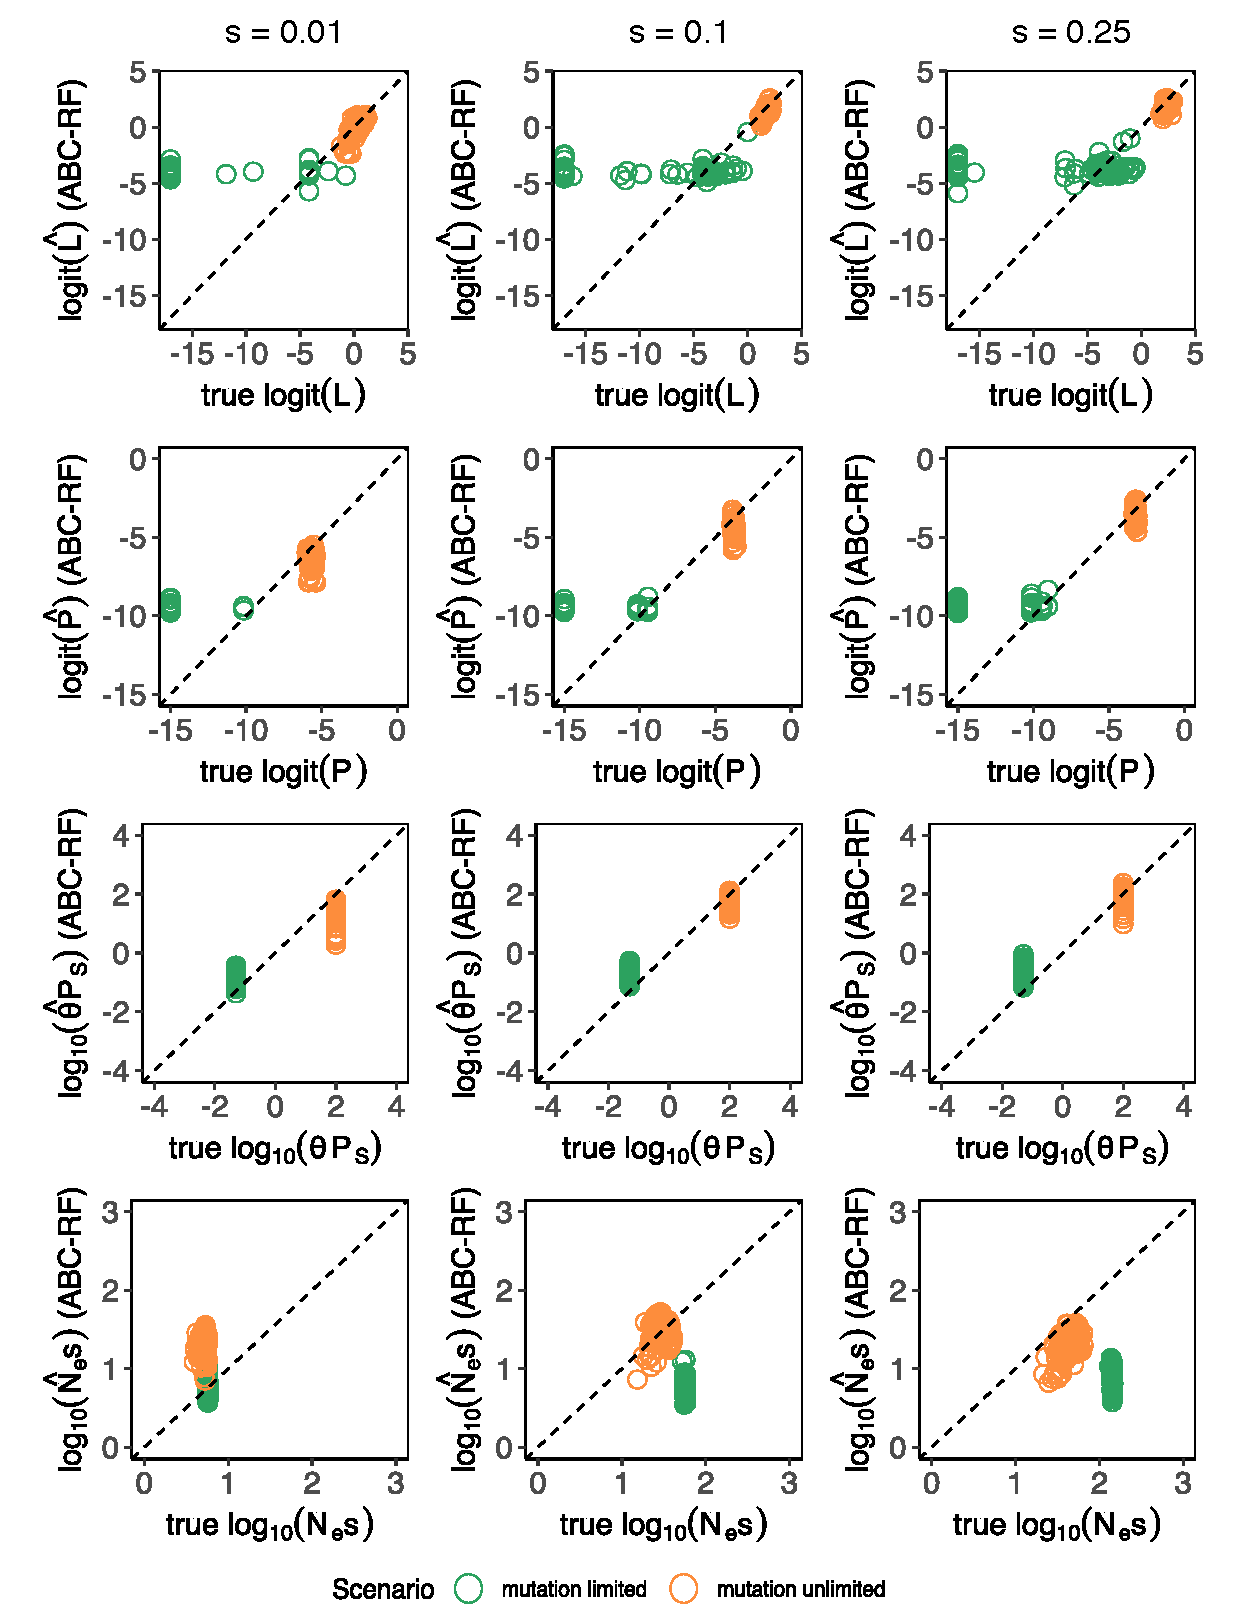
\includegraphics[width=1\textwidth]{Figures/pred_plots_ggplot2_fixed_selection_2.pdf}
  \captionsetup{font=footnotesize}
  \caption{Selection parameters for the constant-values PODs: substitution load $L$, proportion of strongly selected beneficial mutations $P$, scale population size of beneficial mutation $\theta P_{\mathrm{S}}$, and overall strength of selection was calculated as $N_{\mathrm{e}}s$. Comparison between adaptation mutation limited and unlimited scenarios with varying degrees of selection.}
\end{figure}

\begin{figure}[!htb]
  \centering
  \label{fig:fig4}
  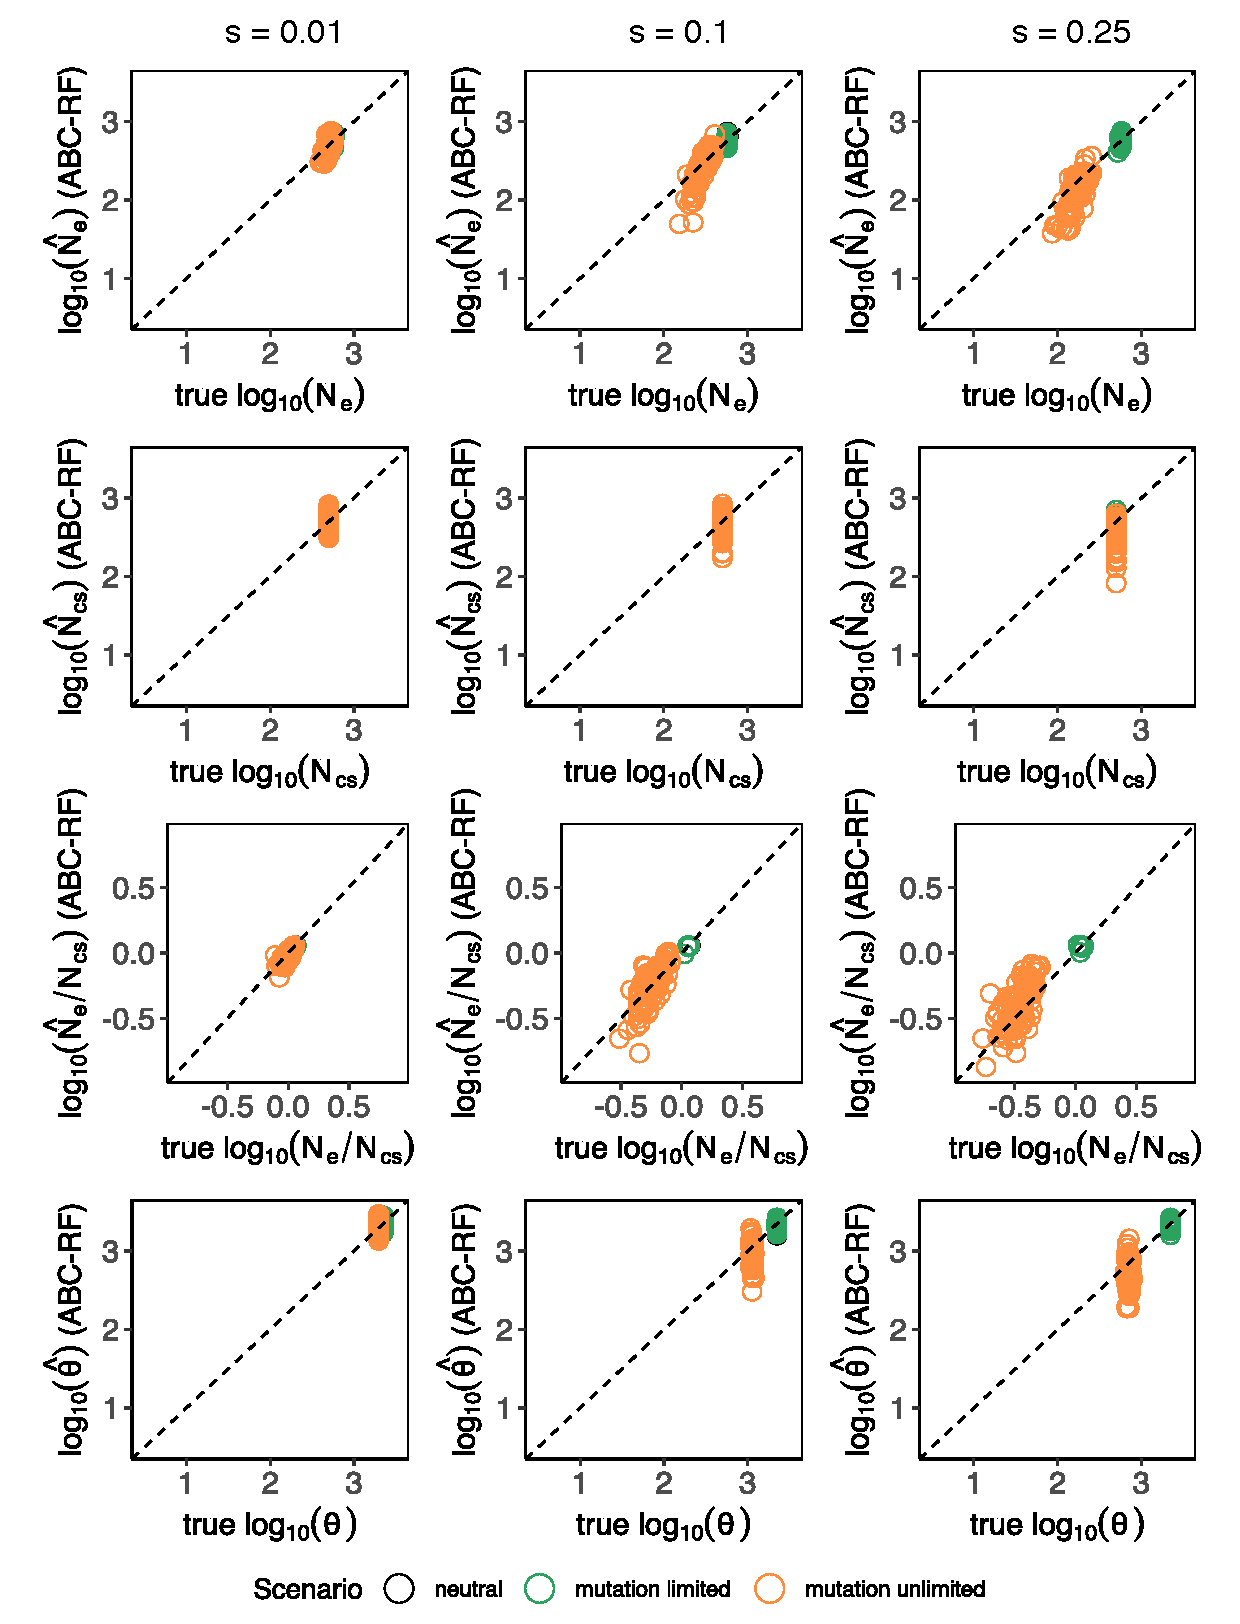
\includegraphics[width=1\textwidth]{Figures/pred_plots_ggplot2_fixed_demog_2.pdf}
  \captionsetup{font=footnotesize}
  \caption{Demography parameters for the constant-values PODs: effective population size $N_{\mathrm{e}}$, population census size $N_{\mathrm{cs}}$, \textbf{(g)} ratio between the effective size and the population census size, and \textbf{(h)} scale population size $\theta$. Comparison between adaptation mutation limited and unlimited scenarios with varying degrees of selection.}
\end{figure}

\begin{figure}[!htb]
  \centering
  \label{fig:fig5}
  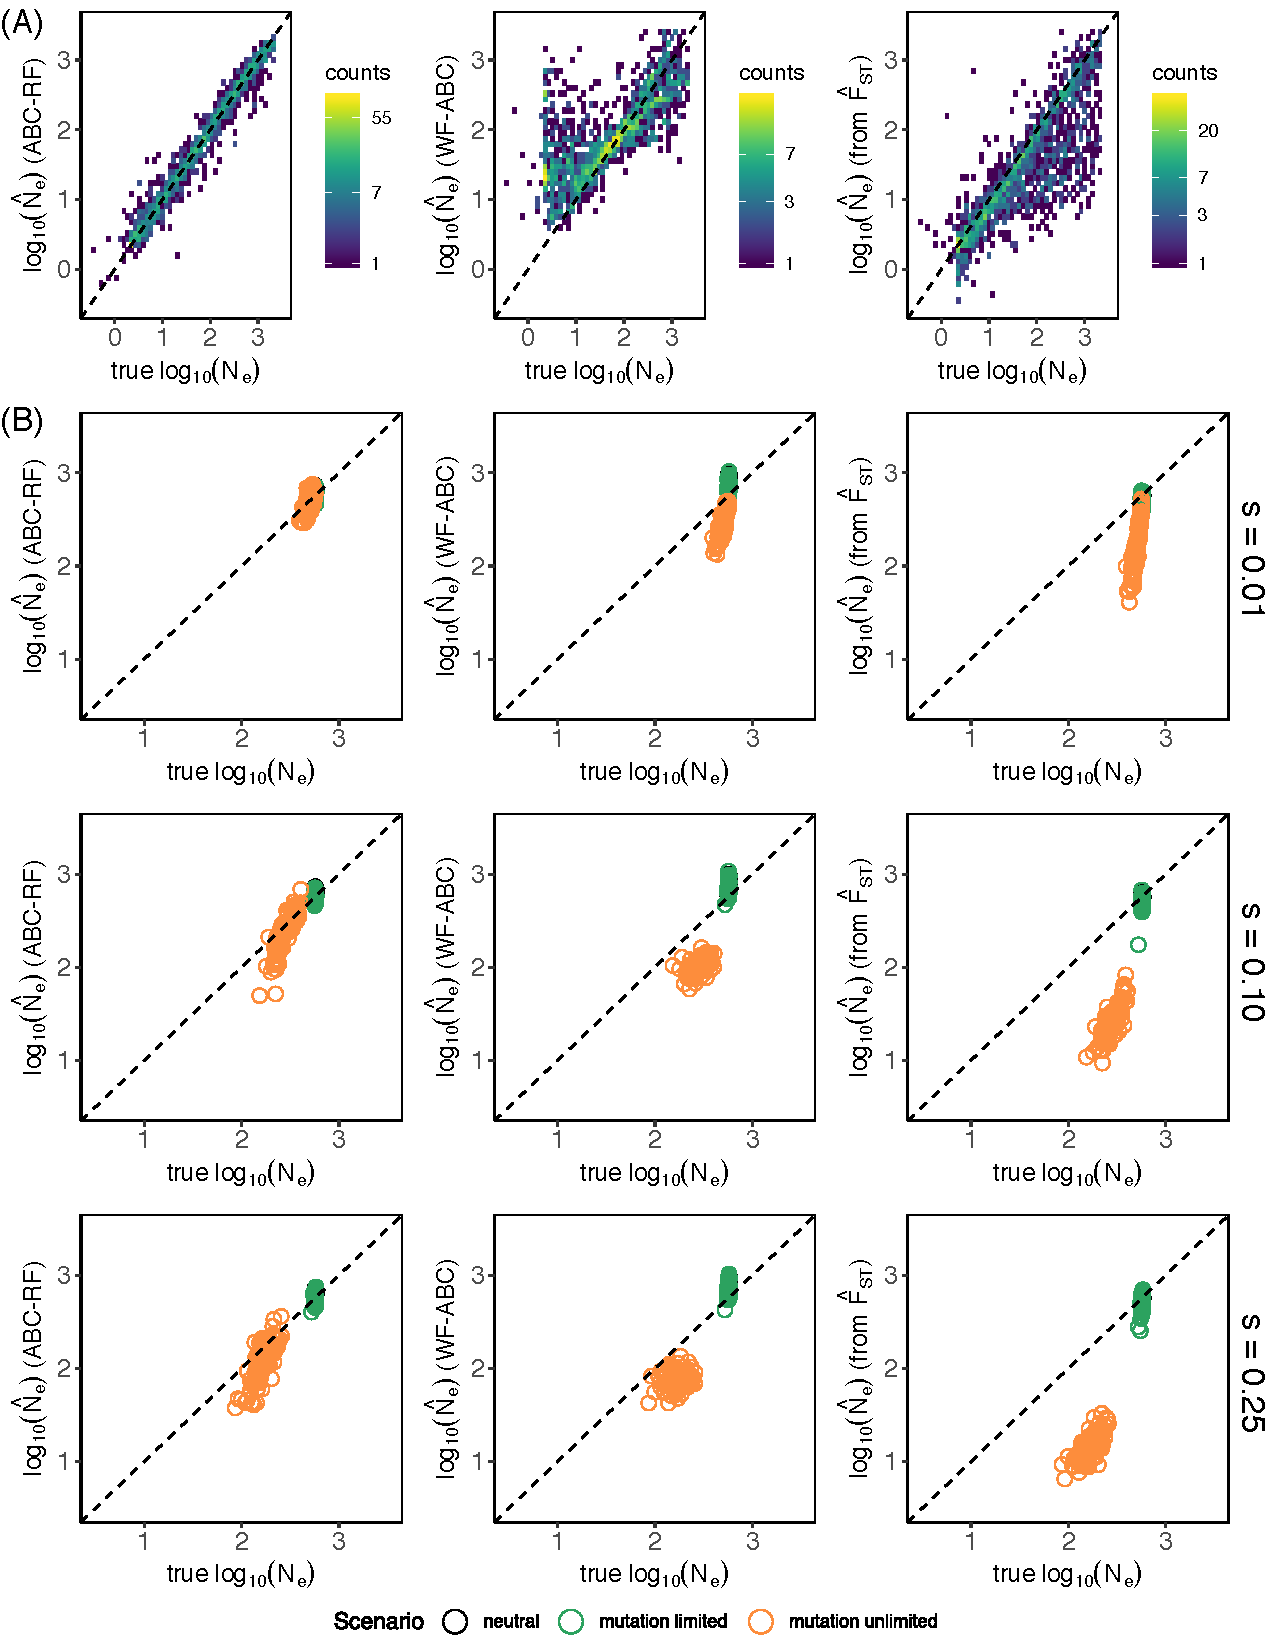
\includegraphics[width=1\textwidth]{Figures/bias_ne_estimates_s_2.pdf}
  \captionsetup{font=footnotesize}
  \caption{Bias of the $N_{\mathrm{e}}$ estimates. \textbf{(A)} ABC-RF, WF-ABC and temporal $F_{\mathrm{ST}}$ for the random-parameter-values PODs; \textbf{(B)} ABC-RF, WF-ABC, temporal $F_{\mathrm{ST}}$ for the constant-values PODs. Comparisons were between adaptation mutation limited and unlimited scenarios with varying degrees of selection.}
\end{figure}

\subsection*{Mutation limited adaptation limits the identification of non-neutral evolution}

We also evaluated the potential of an ABC-RF based classifier to separate the genetic data generated by a neutral/quasi-neutral dynamics or a dynamic where selection is strong and frequent. With the simulations generated to train the ABC-RF, we defined these two discrete classes based on the calculated proportion of strongly selected mutations $P$. We defined as neutral/quasi-neutral simulations those where $P = 0$, and as strong-selection simulations those where $P>0$. Remember that $P$ is dependent on the number of mutations with $s > 1/N_{\mathrm{e}}$ that were present in the population between the sampling time-points. As predicted, our classifier performed well if beneficial mutations were rare and weak, as in a neutral/quasi-neutral dynamics, or if selection was frequent. The global error rate was 19.36 \% for the classification of the data used to train the ABC-RF; the error classification for each class was similar, with 17.94\% of times true neutral/quasi-neutral scenarios wrongly classified as strong-selection, and true strong-selection scenarios wrongly classified as neutral/quasi-neutral. The same patters were observed for the method evaluation on random-parameter-values PODs (Table 3). 

The classification of the three discrete scenarios showed that neutral and mutation unlimited simulations were 100\% correctly classified, but an erroneous classification happened in the mutation limited scenario. In this scenario, the highest global error rate occurred when the average selection coefficient was 0.25, with a global error of 47\%. Figure 5 shows the relationship of the error in the classification of neutral/quasi-neutral scenarios to the values of the scale population size of beneficial mutations $\theta P_{\mathrm{S}}$. When $\theta P_{\mathrm{S}} > 1$ or when $\theta P_{\mathrm{S}} << 0$ the error rate was 0. As for the parameter estimation, scenarios where the sweep was less frequent or rare, as in hard selective sweep of adaptation mutation limited, the few beneficial mutations that arose either swept in the population to fixation or were lost. Even if the beneficial mutations were lost, they left a genome footprint. But, when no beneficial mutation was present to calculate the population $P$, it received a zero value. In mutation limited scenarios, the majority of simulations were affected in some degree by few strong beneficial mutations but, the realized proportion was zero, causing an increase on the classification error.

\begin{table}[ht]
\centering
  \begin{threeparttable}
   \caption{Classification error rate.}
   \label{table:table3}
     \begin{tabular}{lccc}
     \toprule
      Dataset               & Global error rate  & \multicolumn{2}{c}{Class error rate} \\
        {}                  & {}                 & qNeutral as sSel & sSel as qNeutral  \\
     \midrule
      RF-simulations        & 19.36\%$^*$        & 17.94\%          & 20.63\%           \\
      Random PODs           & 19.45\%            & 18.79\%          & 20.02\%           \\
      Fixed PODS            &                    &                  &                   \\
      Neutral               & 0\%                & 0\%              & 0\%               \\
      Mutation limited      &                    &                  &                   \\
         1) s=0.01          & 4\%                & 1\%              & 100\%             \\
         2) s=0.10          & 36\%               & 8.57\%           & 100\%             \\
         3) s=0.25          & 47\%               & 23.40\%          & 72\%              \\
      Mutation unlimited    &                    &                  &                   \\
         1) s=0.01          & 0\%                & 0\%              & 0\%               \\
         2) s=0.10          & 0\%                & 0\%              & 0\%               \\
         3) s=0.25          & 0\%                & 0\%              & 0\%               \\
     \bottomrule
     \end{tabular}
     \begin{tablenotes}
      \small
      \item $^*$ OOB prior error rate.
     \end{tablenotes}
  \end{threeparttable}
  \label{tab:tab3}
\end{table}

\begin{figure}[ht]
  \centering
  \label{fig:fig6}
  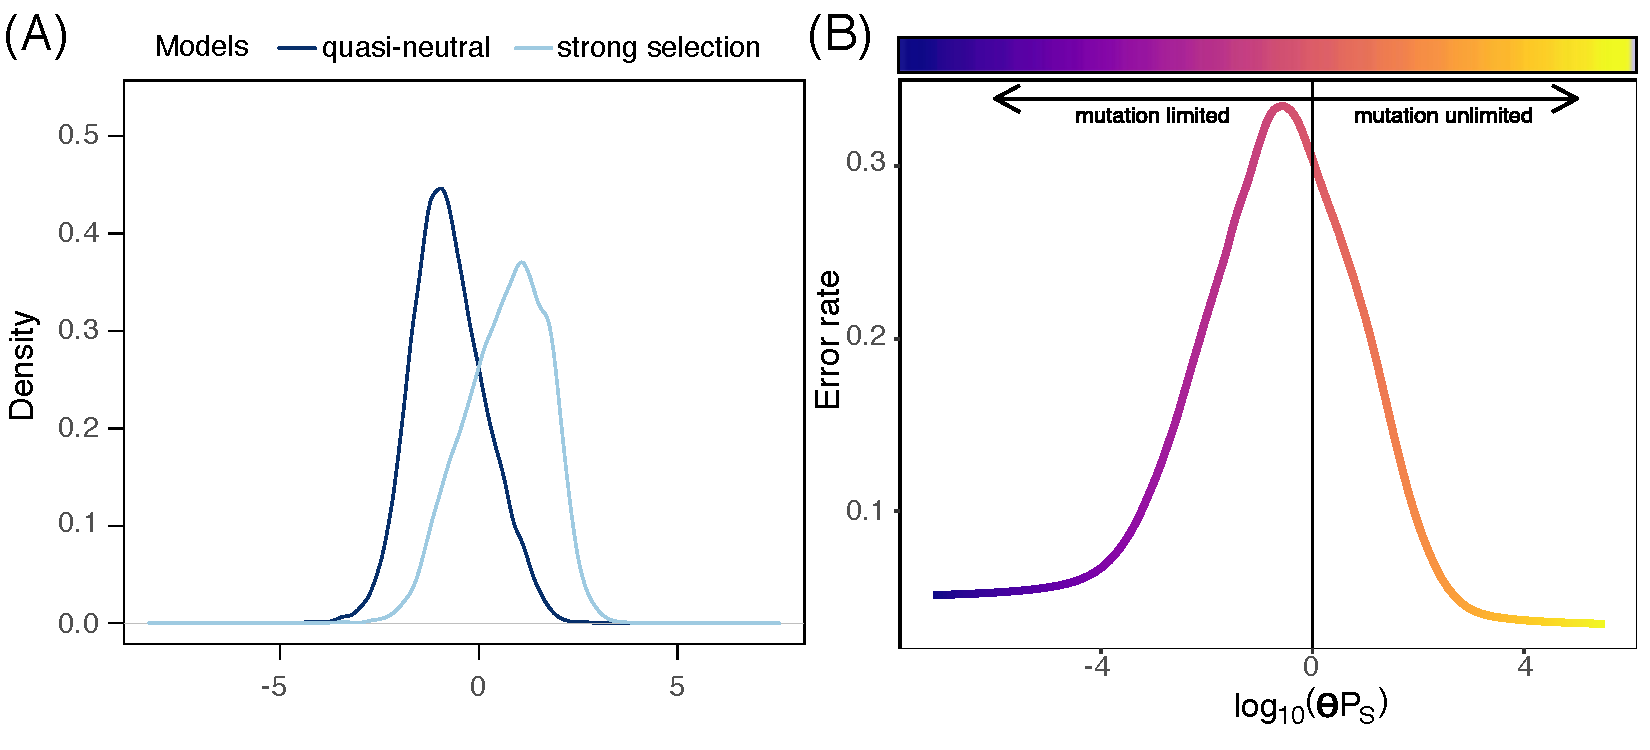
\includegraphics[width=0.95\textwidth]{Figures/lda_class_thetaPS.pdf}
  \captionsetup{font=footnotesize}
  \caption{ABC-RF for classification. \textbf{(A)} density distribution of the linear discrimination predictors of the classification,  \textbf{(B)} the RF classification error rate calculated for windows of $\theta P_{\mathrm{S}}$. The cross-correlation of the error rates and $\theta P_{\mathrm{S}}$ showed that the erroneous of classifications in either selection or neutrality were higher for values of $\theta P_{\mathrm{S}}$ of adaptation mutation limited ($\theta P_{\mathrm{S}}$ << 1). For extreme values of $\theta P_{\mathrm{S}}$ the ABC-RF classifier was able to discriminate between the quasi-neutral and strong-selection scenarios.}
\end{figure}

\begin{figure}[ht]
  \centering
  \label{fig:fig7}
  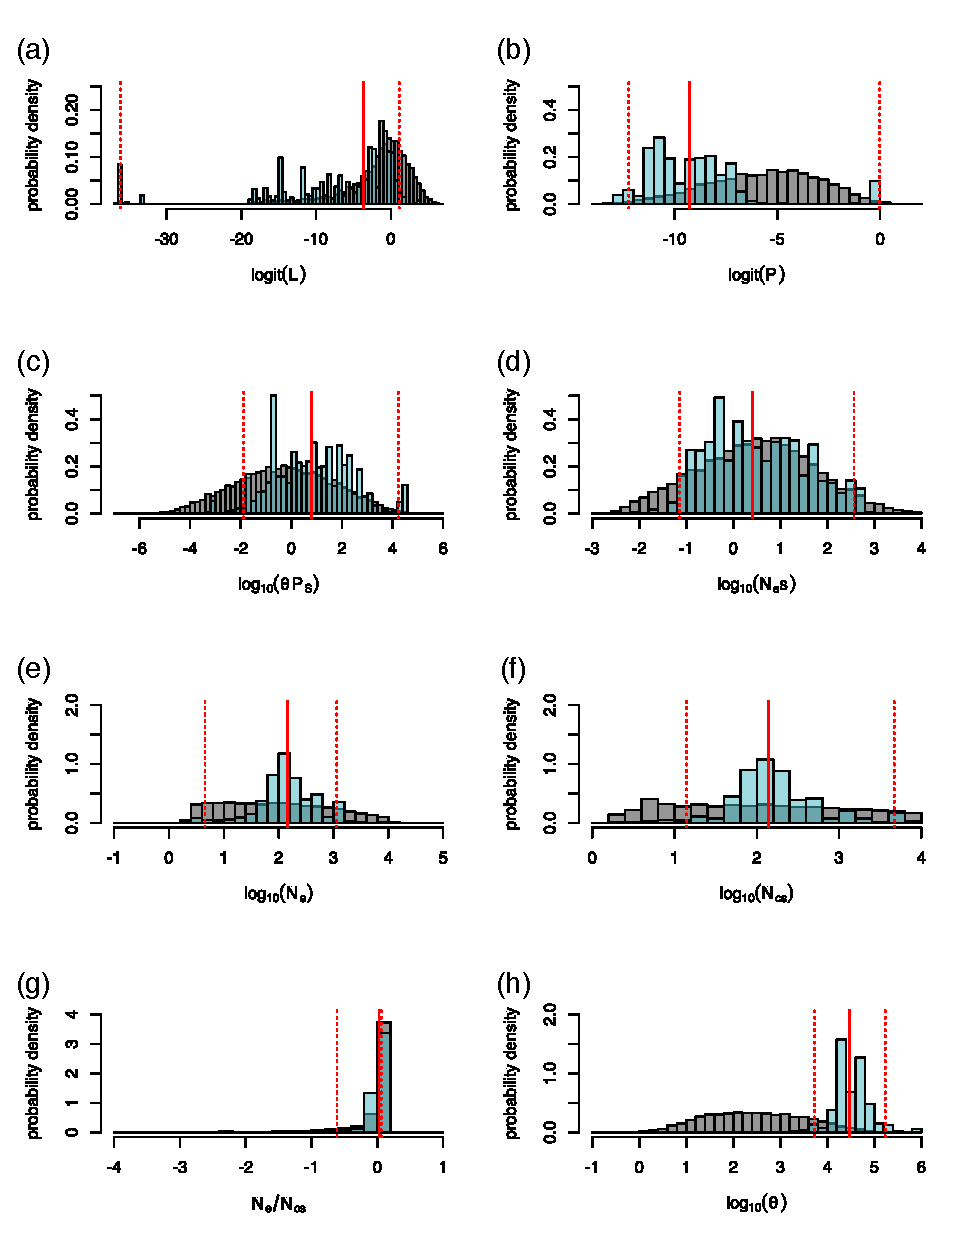
\includegraphics[width=0.95\textwidth]{Figures/pred_prior_post_placerita_mod.pdf}
  \captionsetup{font=footnotesize}
  \caption{Application of the ABC-RF based estimators for demography and selection inference.}
\end{figure}

\subsection*{Dataset}

We applied our ABC-based RF framework to a temporal genomic data of feral population of \textit{Apis mellifera}. This dataset consisted of SNPs variation obtained with whole-genome sequencing of museum and contemporary specimens \citep{Cridland:2018fx}. To exemplify the use of our approach, we selected a population from which a reasonable number of samples were taken in each time-point. For the analysis of this population, we modified the original model to fit the time-span between the two samples and the number of samples taken in each point. The calculation of the genome-wide summary of statistics of each simulation was obtained with the same number of individuals as in the dataset. With only  ~15,000 simulations, we were able to have a pattern of the distribution of the true and predicted values for the training set, similar to the trained RF for the analysis of the PODs (Figure S7). 

When we applied the trained ABC-RF for demographic parameters, we were able to estimate the $N_{\mathrm{e}}$, the $N_{\mathrm{cs}}$ and $\theta$. With our approach, we had similar estimates of the $N_{\mathrm{e}}$ and $N_{\mathrm{cs}}$, with 143.61 and 134.96 individuals, respectively. The temporal $F_{\mathrm{ST}}$ estimator calculated the $N_{\mathrm{e}}$ as 67.77 individuals. It is important to note that we did not model the specificity of the reproductive biology of bees and we were aware that our estimate of $N_{\mathrm{e}}$, that did not take into account this specificity, is naturally overestimated \citep{Nomura:2012bp}. But, we had an estimate in the same order of magnitude as expected for hymenopterans \citep{Zayed:2004kg}. The goal here was not to have an accurate estimation of $N_{\mathrm{e}}$, but to show that our approach can jointly estimate demography and selection, even in datasets of species with limited genomic information.

As a consequence of using a dataset of a species with small $N_{\mathrm{e}}$, we are naturally in a system which adaptation is mutation limited. For this reason, we only had a satisfactory estimate for the proportion of strongly selected mutations. As showed in figure 7, the proportion of mutations under strong selection was $<< 0.1$. This result combined with the estimates of substitution load and $\theta P_{\mathrm{S}}$, showed that the data came from a dynamic of adaptation that was mutation limited. The wider intervals for the estimates of selection parameters lies in the fact that our approach works best in scenarios where adaptation is no limited by mutation. 

Our ABC-RF classifier for this scenario had a global error rate of 28.31\%, slightly higher than for the analysis of the PODs. However, with a classification error of 18.27\% for neutral scenarios classified as strong selection, and 38.36\% for strong selection scenarios classified as neutral/quasi-neutral. When we applied the classifier to the dataset, it determined it as a neutral/quasi-neutral dynamics. Despite the lower performance compared to the PODs, we were still able to learn about the selection dynamics of a feral A. mellifera population and a $N_{\mathrm{e}}$ when selection was taken into account.

\subsection*{Perpectives and Limitations}

We developed an ABC-based framework to jointly infer genome-wide demography and selection parameters on whole-genome sequencing temporal data. In our model, we were able to take into account the pervasive effect of selection, as in recurrent hitchhiking models (RHH). We showed that for the demographic inference, the pervasiveness and strength of selection has a limited impact in our ABC-RF approach. We also showed that in the parameter space that defined adaptation as not limited by mutation, the ABC-RF approach satisfactorily inferred genome-wide parameters of the adaptive history, regardless the strength of selection. But, our approach had a limitation on scenarios where adaptation was less frequent. 

Our model is very simplistic, as it did not consider the impact of mutations with a negative selection coefficient, such as in background selection models. Background selection can mimic directional selection by determining a similar pattern of diversity reduction around the target of selection. However, it was recently shown that background selection only mimic the classic sweep in simplistic models, where the deleterious mutation is localized in a specific region of the genome \citep{Schrider:2019ih}. For more realistic scenarios, where the concentration of deleterious mutations varies across the genome, background selection do not behave as a classic sweep. In an attempt o jointly accommodate the effect os demography and selection on the inference of $N_{\mathrm{e}}$,  \citet{Johri:2019jv} modeled the effect of background selection and developed an ABC-based approach that jointly estimated the distribution of fitness effects (DFE) and $N_{\mathrm{e}}$. In their simulations, deleterious mutations were modeled more realistically. They also included some beneficial mutations, similarly to a classical hard sweep. They showed an unbiased estimate of $N_{\mathrm{e}}$ regardless the presence of positive and negative selection. But, based on what we have showed, is not the strength but the frequency of positive selection that bias $N_{\mathrm{e}}$.
It is important to measure the impact of deleterious mutations more realistically together with recurrent hitchhiking selection.

An important development of our approach is to model more realistic scenarios in which selection acts on standing genetic variation. This can be easily achieved with our pipeline and allows for a more general treatment of selection of soft sweeps. In addition, we are aware that more complex demographic scenarios should be evaluated and that our model should be expanded to explore hard selection that can be modeled outside the traditional Wright-Fisher models \citep{Haller:2019cy}.

\section*{Conclusion}
We show how increasing selection affects the estimates of the effective population size $N_{\mathrm{e}}$ and how different it can be from the population census size $N_{\mathrm{cs}}$. With our ABC-RF approach on temporal genomic data, we show an unbiased estimate of $N_{\mathrm{e}}$, regardless the strength or pervasiveness of selection. We also show that additional selection and demographic parameters can be obtained with and ABC-RF based inferential approach. Parameters as substitution load, the rate of adaptive mutation and the proportion of beneficial mutation segregating in the population were traditionally obtained with additional genomic and functional genomic information. For the first time, we show an approach that does not depend on this information and that can be used in the study of organisms that do not have detailed genomic information.

\bibliographystyle{apalike}
\bibliography{references}
\end{document}